\documentclass{beamer}
\usepackage{graphicx}
\usetheme{Berlin}

\begin{document}

\begin{frame}
\frametitle{Music-Reactive RGB LEDs Circuit}
\framesubtitle{Introduction}
\begin{center}
\textbf{Title: Music-Reactive RGB LEDs Circuit}
\end{center}
\end{frame}

\begin{frame}
\frametitle{Music-Reactive RGB LEDs Circuit}
\framesubtitle{Presented By}
\begin{itemize}
  \item Presented By:
  \item Naveed Ahmad
  \item Muhammad Kamil Khan
  \item  Sharjeel Qureshi
\end{itemize}
\end{frame}

\begin{frame}
\frametitle{Music-Reactive RGB LEDs Circuit}
\framesubtitle{What is a Music-Reactive RGB LEDs Circuit?}
\begin{itemize}
  \item Introduction
  \item A music-reactive RGB LED circuit combines RGB LEDs and audio input to produce visually captivating light displays.
  \item These circuits respond to sound levels and frequencies, transforming them into dynamic lighting effects that follow the rhythm of the music.
  \item The LEDs turn on and off according to the music pattern.
\end{itemize}
\end{frame}

\begin{frame}
\frametitle{Music-Reactive RGB LED Circuit}
\framesubtitle{Components}
\begin{itemize}
  \item Components:
  \begin{itemize}
    \item Mic
    \item NPN Transistor (e.g., BC547)
    \item Resistors: 10k (2), 1k (4), 1M (1)
    \item Ceramic Capacitor: 100nF
    \item RGB LEDs
    \item 9V Battery
    \item Breadboard and connecting wires
  \end{itemize}
\end{itemize}
\end{frame}

\begin{frame}
\frametitle{Music-Reactive RGB LED Circuit}
\framesubtitle{Schematic Diagram}
\begin{figure}
  \centering
  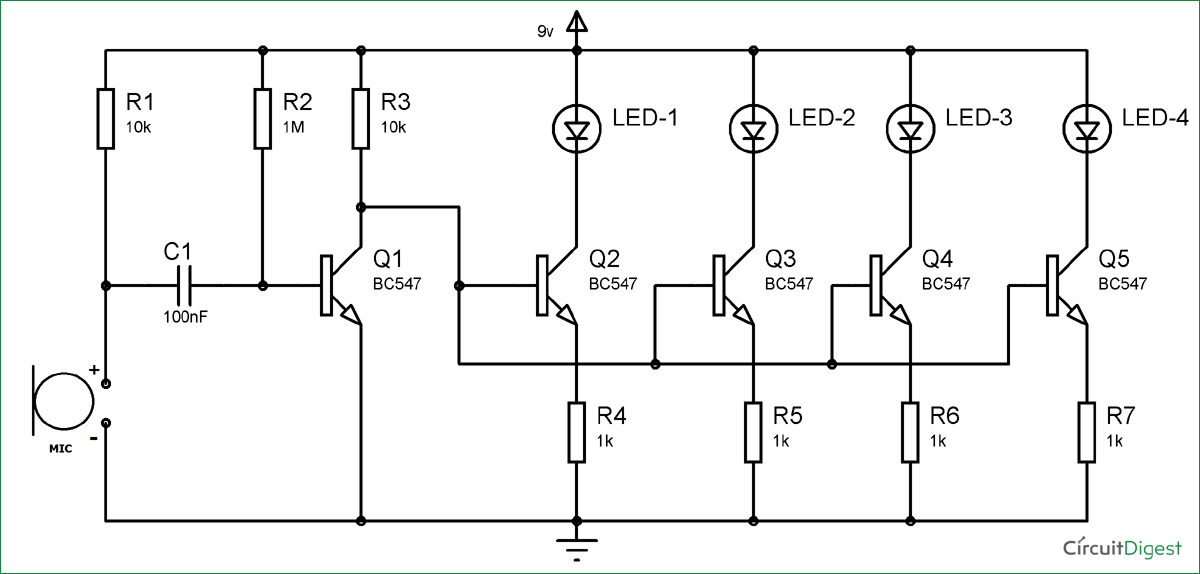
\includegraphics[scale=0.27]{image1.png}
  \caption{Schematic diagram}
  \label{fig:image1}
\end{figure}
\end{frame}

\begin{frame}
\frametitle{Music-Reactive RGB LED Circuit}
\framesubtitle{How Does It Work?}
\begin{itemize}
\item Works in four steps:
 \item (I) Sound Input:
 \item (II) Noise Filtering:
 \item (III) Signal Amplification:
 \item (IV) LEDs Activation:
  
  
\end{itemize}
\end{frame}

\begin{frame}
\frametitle{Music-Reactive RGB LED Circuit}
\framesubtitle{Sound Input}
\begin{itemize}
  \item Sound Input:
  \item The circuit uses a condenser microphone to pick up sound signals and convert them into voltage levels.
  \item  The microphone acts as a sensor that captures the surrounding sound.
  \item The microphone converts sound signals into varying voltage levels.
  
\end{itemize}
\end{frame}

\begin{frame}
\frametitle{Music-Reactive RGB LED Circuit}
\framesubtitle{how Mic convert sound signal into voltage levels?}
\begin{itemize}
  \item The microphone consists of a diaphragm and a transducer.
  \item Sound waves cause the diaphragm to vibrate, changing the capacitance of the transducer.
  \item The changing capacitance generates an electrical signal that represents the sound.
  \item The electrical signal from the microphone is in the form of varying voltage levels corresponding to the sound waves.
\end{itemize}
\end{frame}

\begin{frame}
\frametitle{Simple LED Music Light Circuit}
\framesubtitle{Noise Filtering}
\begin{itemize}
  \item Noise Filtering:
  \item To remove any unwanted noise from the sound signals, a high-pass filter is used.
  \item The filter consists of a resistor (R2) and a capacitor (C1).
  \item This filter allows higher frequency components associated with the music or sound to pass through while blocking lower frequency noise.
\end{itemize}
\end{frame}

\begin{frame}
\frametitle{Simple LED Music Light Circuit}
\framesubtitle{Signal Amplification}
\begin{itemize}
  \item Signal Amplification:
  \item The filtered signals are then amplified using an NPN transistor (Q1).
  \item The transistor acts as an amplifier, boosting the strength of the signals for further processing.
\end{itemize}
\end{frame}

\begin{frame}
\frametitle{Simple LED Music Light Circuit}
\framesubtitle{LEDs Activation}
\begin{itemize}
  \item LEDs Activation:
  \item The amplified signals are fed into an array of transistors.
  \item Each transistor in the array acts as an amplifier as well.
  \item When the amplified signals pass through the transistors, they trigger the corresponding LEDs to light up.
  \item Each transistor in the array works as an amplifier, causing the LEDs to glow based on the sound pattern.
  \item Additional LEDs can be added with transistors to enhance the visual effect.
  \item Based on the analyzed data, the intensity or color of the RGB LEDs changes, creating synchronized lighting effects.
\end{itemize}
\end{frame}

\end{document}
